\section{Sicherheitskonzept von WhatsApp}\label{sec:kaptiel}
\cite{ENCOV}Das Sicherheitskonzept, welches von WhatsApp bereitsgestellt wird, zeigt wie
der Nachrichtenausstausch 'Ende-zu-Ende' verschlüsselt wird. Dabei wird neben
den verschiedenen Verschlüsselungs-Verfahren auch der Austausch der Nachrichten
dargestellt, die zur Registrierung bei WhatsApp, zur Anmeldung mit einem neuen
Endgerät, sowie dem eigentlich Austausch von Nachrichten, Sprachnachrichten, Bildern
und Videos notwendig sind. 
Um diesen Nachrichtenaustausch später analysieren zu können, werden die Konzepte
von WhatsApp kurz dargestellt.\cite{ENCOV}; 

WhatsApp ist nicht auf Verschlüsselungs spezialisiert. Deswegen verwendet WhatsApp
die Krypto-Suite 'Open Whisper Systems'. Diese Suite wird nicht nur von WhatsApp verwendet, 
sondern auch von 'Signal'.
'Open Whisper Systems'-Suite bietet eine Ende-zu-Ende-Verschlüsselung an. Das Ziel
ist, dass weder Dritte noch WhatsApp selbst Zugriff auf die Klartext-Nachrichten haben.
Dies soll auch bei Verlust oder Veröffentlichung des privaten Schlüssels der Fall sein, 
das heißt mit einem bekannten Private Key können vergangene und zukünftige Nachrichten
nicht entschlüsselt werden können. Um dies zu erreichen verwendet WhatsApp eine 
Vielzahl von verschiedenen Schlüsseln die sich unterteilen in Public Keys und Session Keys. 

\underline{Public Key Types: }
    \begin{itemize}
        \item Identity Key Pair: langzeit, Curve25519, erstellt bei Installation 
        \item Signed Pre Key: Curve25519, erstellt bei Installation, signiert von Identity Key, rotiert zeitbasiert
        \item One-Time Pre Key: mehrere Curve25519, erstellt bei Installation, ergänzt falls notwendig
    \end{itemize}
    
\underline{Session Key Types:}
    \begin{itemize}
        \item Root Key: 32 bit, verwendet um Chain Key zu erstellen
        \item Chain Key: 32 bit, verwendet um Message Key zu erstellen
        \item Message Key: 80 bit, verwendet um die Nachricht zu verschlüsseln 
    \end{itemize}

Die Nachrichten werden mit dem 'Message Key' verschlüsselt, dieser besteht aus einem 32 bit AES-256 Key (im CBC-Mode), einer 32 bit HMAC-SHA256 Key Signatur und einem 16 bit Initialisierungsvektor. 
Der Message Key ist flüchtig, das heißt er wird für jede Nachricht die übertragen wird, neu erstellt.
Dies sorgt dafür, dass nach dem Senden bzw. Empfangen der Nachricht dieser nicht mehr 
gültig ist. Gelangt ein Message Key an die Öffentlichkeit, kann so nur eine einzige Nachricht
entschlüsselt werden und eben keine vergangenen oder zukünftigen.
Die HMAC-SHA256 Signature die an den eigentlichen Schlüssel angehängt wird, dient
zur Authentifizierung.

\subsection{TLSv1.3}
\cite{tls} WhatsApp verwendet für die Verschlüsselung der Pakete TLSv1.3.
Im Vergleich zu TLSv1.2 werden bei der späteren Analyse weniger Pakete erwartet.
In der Folgenden Darstellung wird gezeigt, was sich im Vergleich zu 
TLSv1.2 verändert hat. 

\begin{center}
    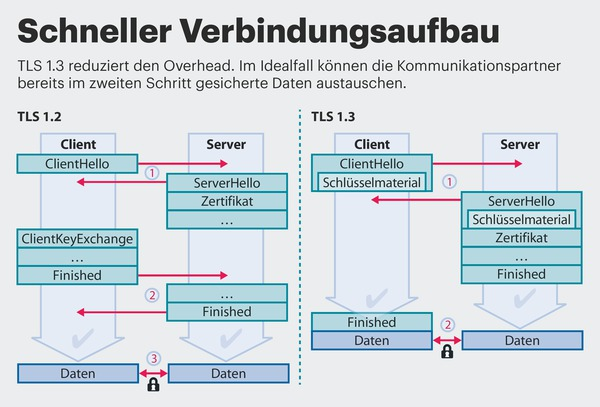
\includegraphics[width=10cm]{tlsv13}
\end{center}
Mit TLSv1.3 werden einige Pakete nicht mehr benötigt, dies sorgt für einen 
schnelleren Verbindungsaufbau. Zusätzlich wurden auch einige Einschränkungen
getroffen. So wird der Austausch von symmetrischen Schlüsseln über RSA
nicht mehr erlaubt. Verwendet werden soll das Deffie-Hellman-Verfahren, welches
nur geringfügig mehr Aufwand erfordert. Allerdings kann mithilfe von Deffie-Hellman zusätzlich 
sichergestellt werden, dass bei Verlust des Schlüssels, vergangene Nachrichten
nicht entschlüsselt werden können. Wie zuvor beschrieben, ist dies 
ein Prinzip von WhatsApp.
Bei der Analyse von WhatsApp, können demnach bzgl. TLSv1.3 folgende Pakete erwartet werden: 
\begin{enumerate}
    \item \textit{ClientHello}: Mit den Informationen zum Deffie-Hellmann-Schlüsselaustausch
    \item \textit{ServerHello}: Mit den Informationen zum Deffie-Hellmann-Schlüsselaustausch, dem Zertifikat und einem Finished-Flag.
    \item \textit{Finished}: Finished-Flag vom Client und evtl. bereits Applikationsdaten
    \item \textit{Applikationsdaten}: Beliebig viele Pakete zum Austausch von Applikationsdaten
\end{enumerate}
\textbf{Cipher-Suites}\\
\cite{tls2} Für TLSv1.3 stehen bisher 5 Cipher-Suites zur Verfügung: 
\begin{itemize}
    \item \texttt{TLS13-AES-256-GCM-SHA384}
    \item \texttt{TLS13-CHACHA20-POLY1304-SHA256}
    \item \texttt{TLS13-AES-128-GCM-SHA256}
    \item \texttt{TLS13-AES-128-CCM-8-SHA256}
    \item \texttt{TLS13-AES-128-CCM-SHA256}
\end{itemize}
\textbf{Kurzbeschreibung der Abkürzungen:}\\
Dies ist eine kleine Übersicht, die einzelnen Verfahren werden nicht erklärt.
\begin{description}
    \item \texttt{AES}:Advanced Encryption Standard - symmetrisches Verschlüsselungsverfahren
    \item \texttt{CCM}: Counter with CBC-MAC - basiert auf CTR
    \item \texttt{GCM}:Galois/Counter Mode - basiert auf CTR
    \item \texttt{SHA}: Secure Hash Algorithm - kryptographische Hashfunktion
\end{description}







 
